\documentclass{article}
\usepackage{amsmath}
\usepackage{graphicx}

\title{Kepler's Laws}
\author{Madhumitha}

\begin{document}
\maketitle

\section{Introduction}
Johannes Kepler formulated three fundamental laws of planetary motion. These laws describe the motion of planets around the Sun and have been instrumental in our understanding of celestial mechanics. In this document, we will present Kepler's laws and provide a brief explanation of each.

\section{First Law: Law of Ellipses}
\textbf{Law:} Each planet orbits the Sun in an ellipse with the Sun at one of the two foci.

\textbf{Explanation:} According to Kepler's first law, the path followed by a planet around the Sun is not a perfect circle but an ellipse. An ellipse is a closed curve with two foci.The point at which the planet is close to the sun is known as perihelion and the point at which the planet is farther from the sun is known as aphelion. The Sun is located at one of the foci, while the other focus remains empty. This law suggests that the distance between the planet and the Sun varies throughout its orbit.

\begin{figure}[ht]
    \centering
    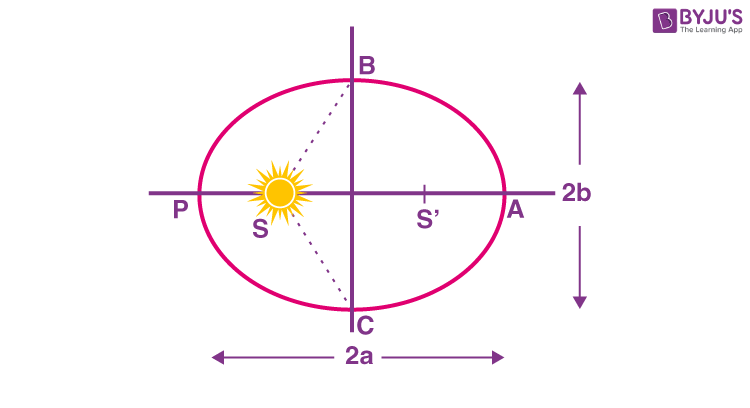
\includegraphics[width=0.5\textwidth]{imag1.jpg}
    \caption{$Kepler's First Law$}
    \label{fig:example}
\end{figure}

\section{Second Law: Law of Equal Areas}
\textbf{Law:} A line connecting a planet to the Sun sweeps out equal areas in equal time intervals.

\textbf{Explanation:} Kepler's second law states that the imaginary line connecting a planet to the Sun sweeps out equal areas in equal time intervals. This means that a planet moves faster when it is closer to the Sun (in the perihelion region) and slower when it is farther away (in the aphelion region). The law implies that the orbital speed of a planet changes as it moves around the Sun.

\begin{figure}[ht]
    \centering
    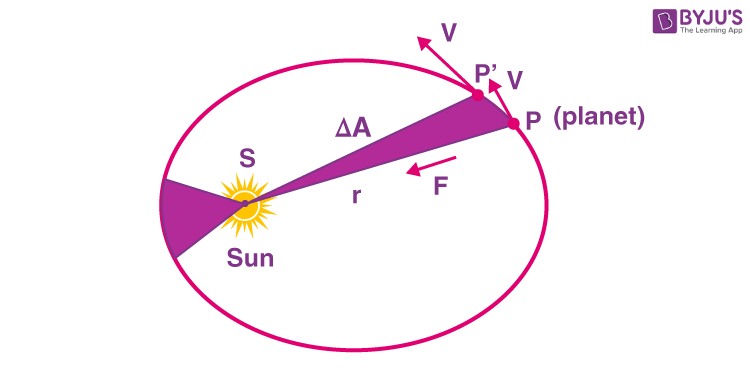
\includegraphics[width=0.5\textwidth]{imag2.jpg}
    \caption{$Kepler's Second Law$}
    \label{fig:example}
\end{figure}

\section{Third Law: Law of Harmonies}
\textbf{Law:} The square of the orbital period of a planet is directly proportional to the cube of its average distance from the Sun.

\textbf{Explanation:} Kepler's third law establishes a relationship between a planet's orbital period and its average distance from the Sun. The law states that the square of the orbital period is proportional to the cube of the semi-major axis of the planet's elliptical orbit. Mathematically, this can be expressed as:
\[
T^2 = k \cdot r^3
\]
where $T$ is the orbital period, $r$ is the average distance from the Sun, and $k$ is a constant. This law allows us to compare the orbital periods and distances of different planets and make predictions about their motions.

\section{Conclusion}

Kepler's laws provide a fundamental framework for understanding the motion of planets in our solar system. They revolutionised our understanding of celestial mechanics and laid the foundation for Isaac Newton's laws of motion and universal gravitation.
\footnote{byjus:Kepler's Laws of Planetary Motion}


\textbf{Name:} Madhumitha

\textbf{github user-id:} MadhumithaSRMS

\end{document}

